\section{แผนผังการทำงานแบบลำดับปฏิสัมพันธ์ (Sequence Diagram)}
การออกแบบแผนผังการทำงานแบบลำดับปฏิสัมพันธ์ ดังนี้

\begin{figure}
    \makebox[\textwidth][c]{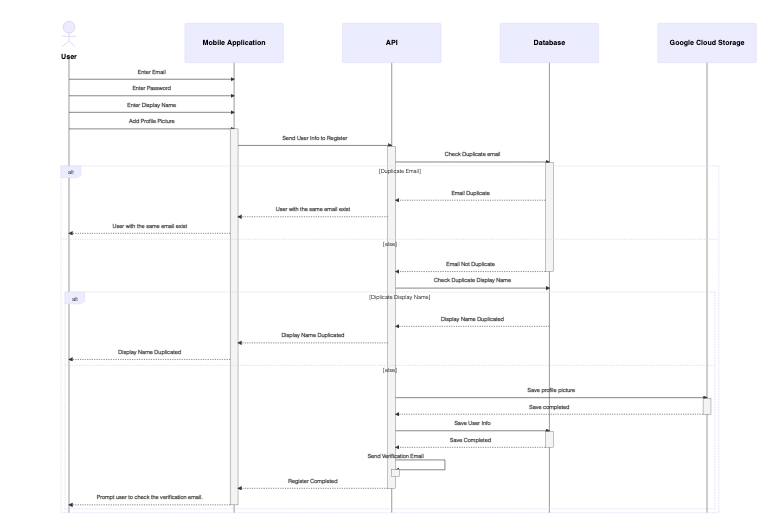
\includegraphics[width=\paperwidth - 3cm]{chapter_3/sequence/Register-1.md.png}}
    \caption{การทำงานในส่วนการลงทะเบียนผู้ใช้}
\end{figure}

\begin{figure}
    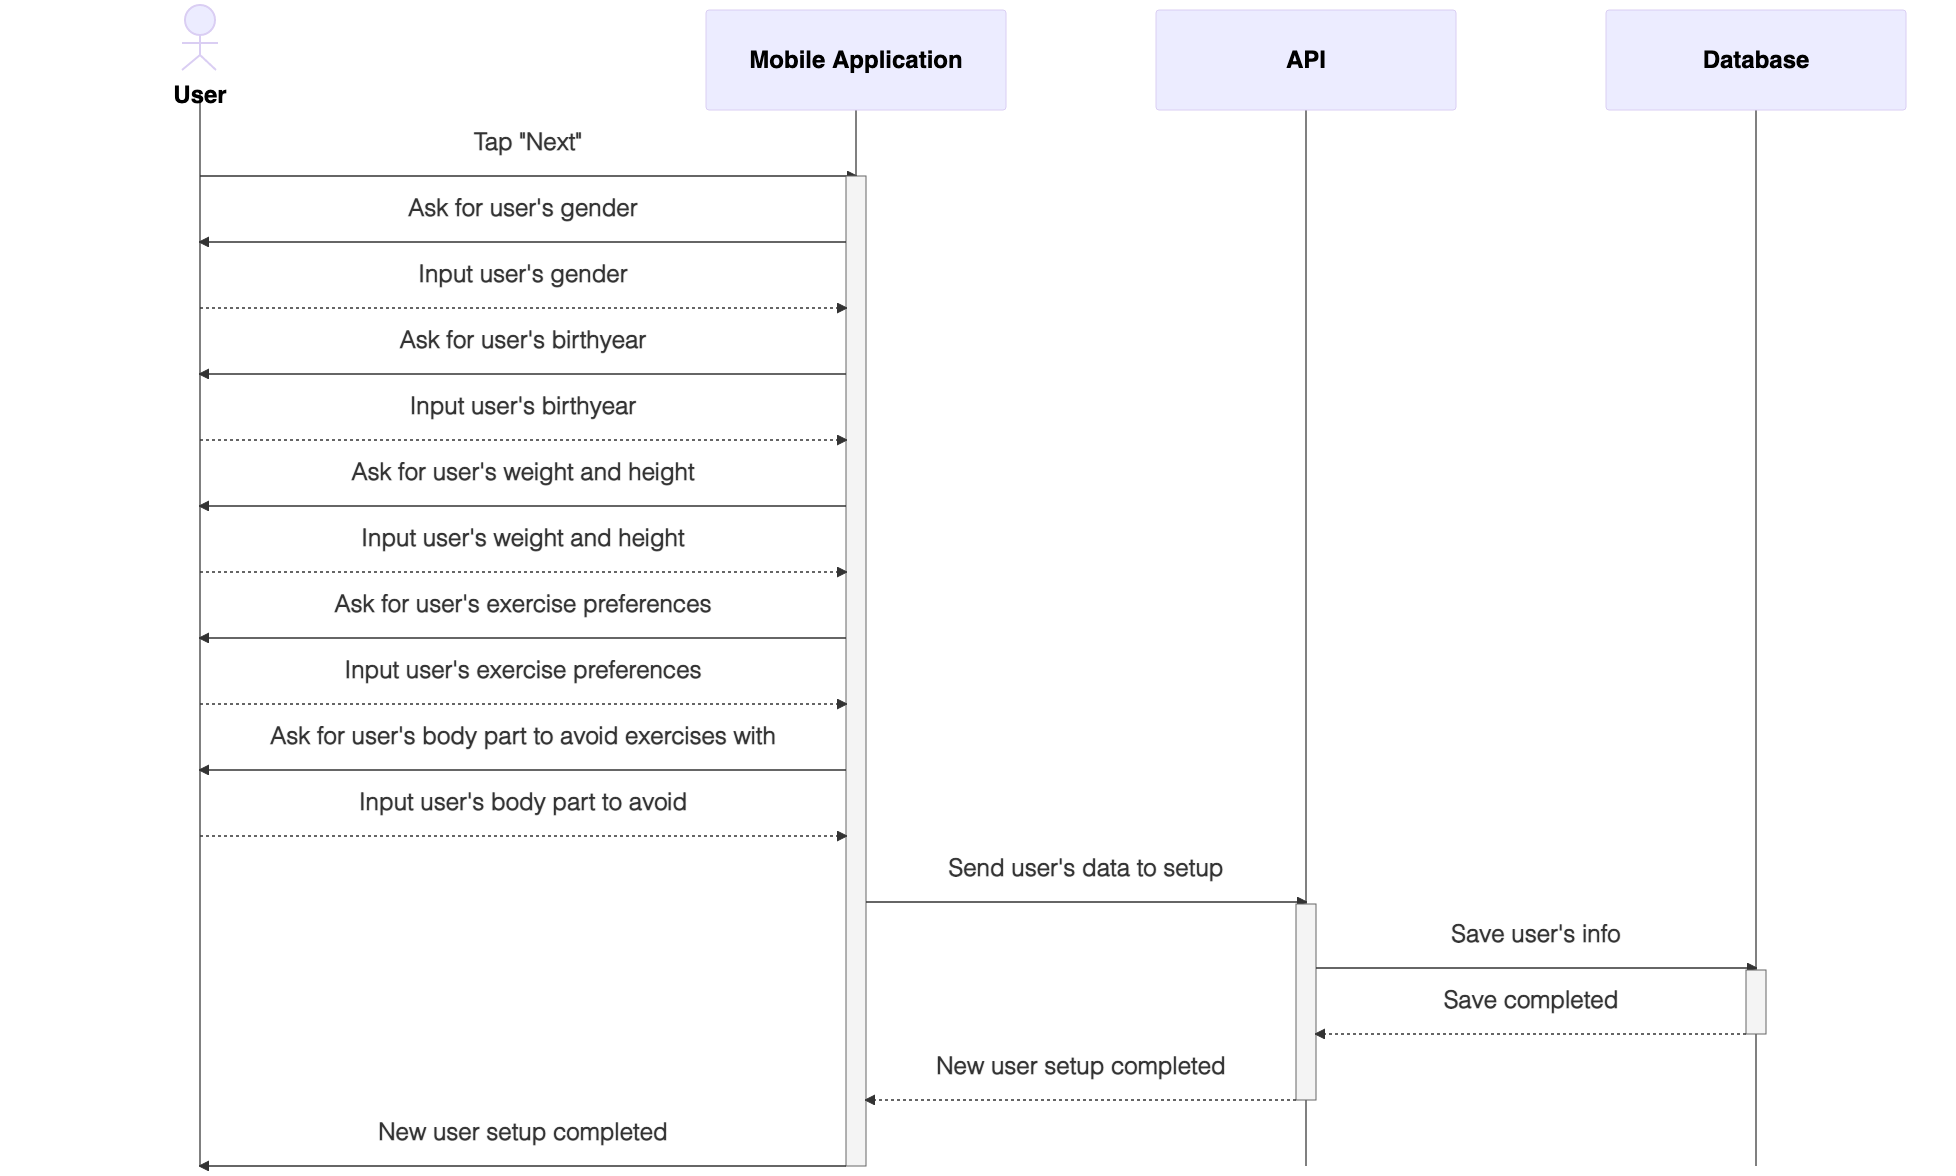
\includegraphics[width=\textwidth]{chapter_3/sequence/New User Setup-1.md.png}
    \caption{การทำงานในส่วนการตอบคำถามความต้องการออกกำลังกาย}
\end{figure}

\begin{figure}
    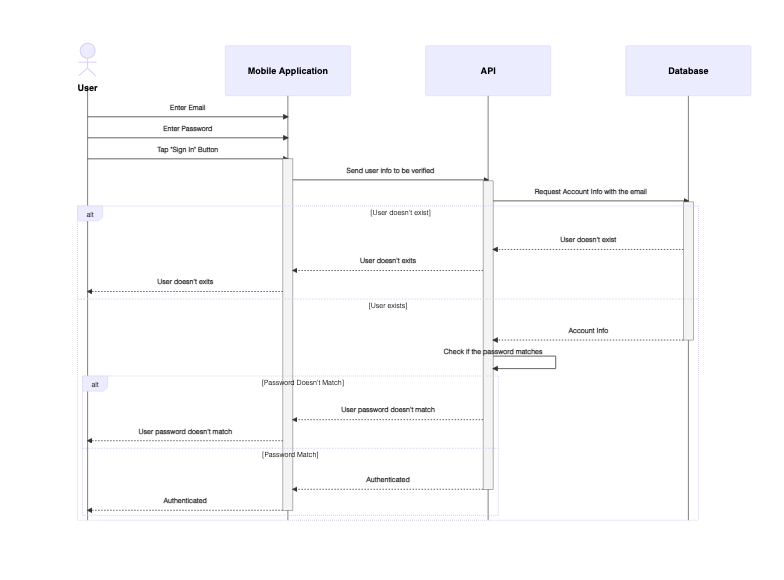
\includegraphics[width=\textwidth]{chapter_3/sequence/Sign In-1.md.png}
    \caption{การทำงานในส่วนการเข้าสู่ระบบ}
\end{figure}

\begin{figure}
    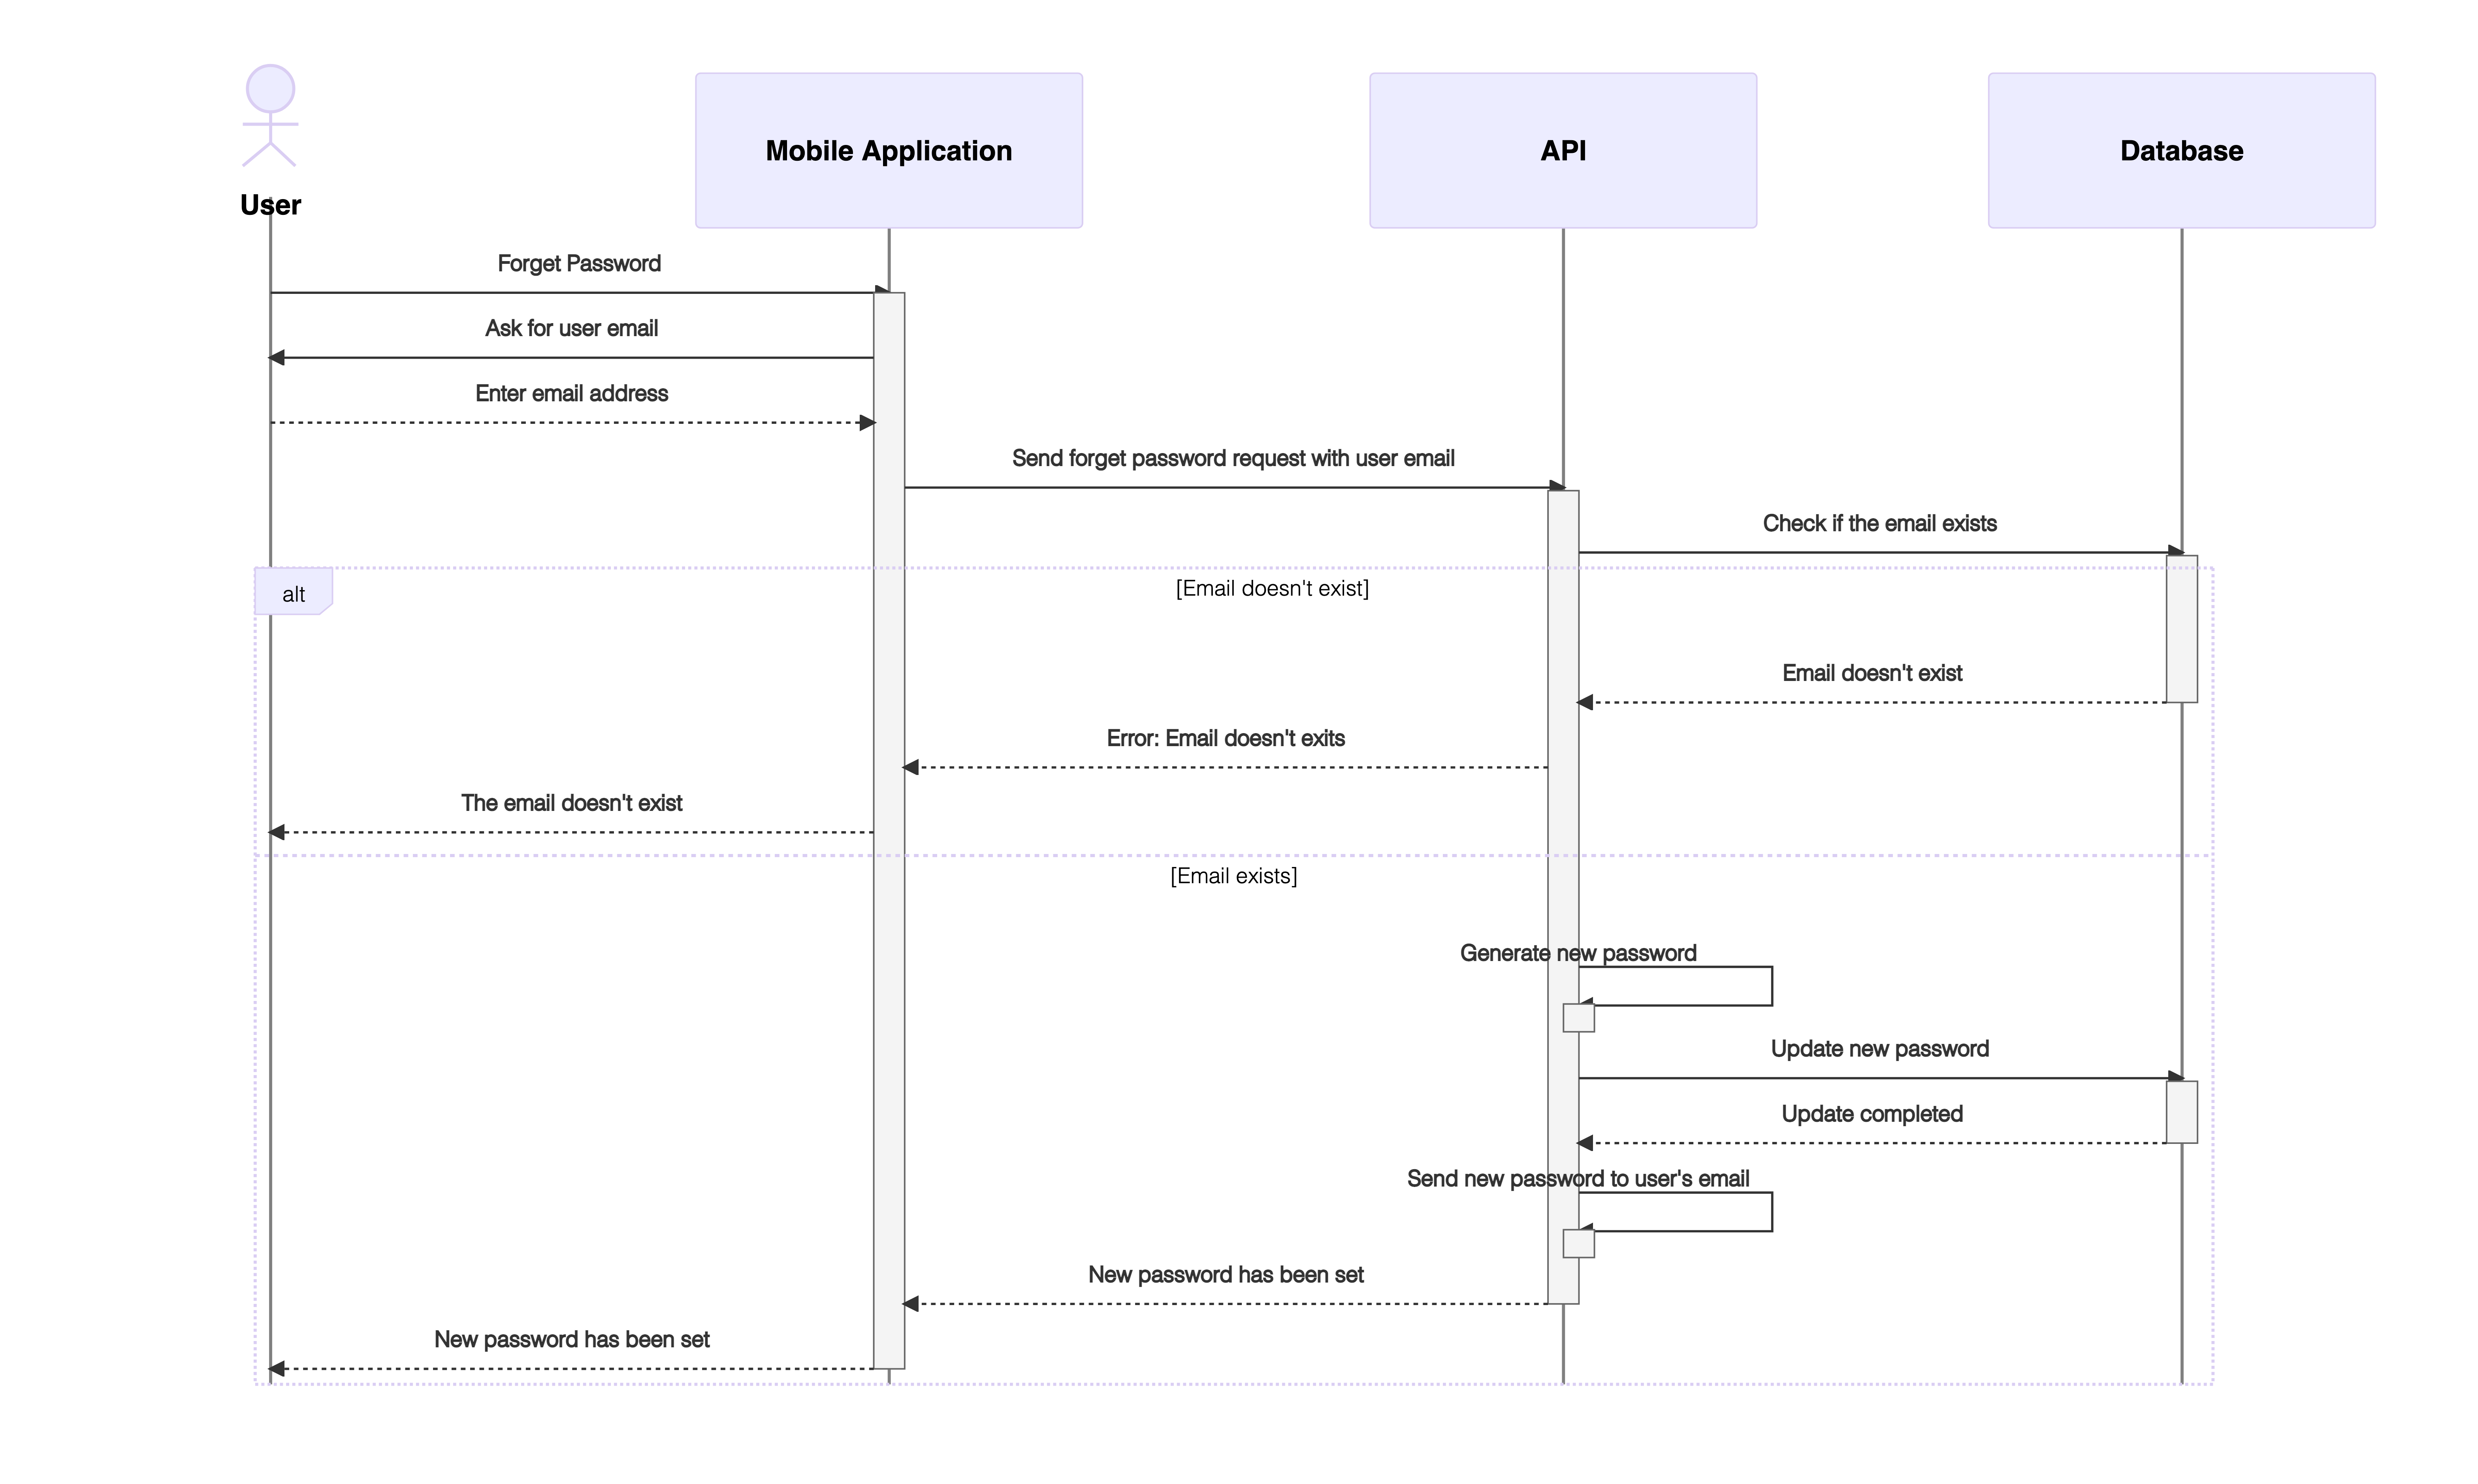
\includegraphics[width=\textwidth]{chapter_3/sequence/Forget Password-1.md.png}
    \caption{การทำงานในส่วนการลืมรหัสผ่าน}
\end{figure}

\begin{figure}
    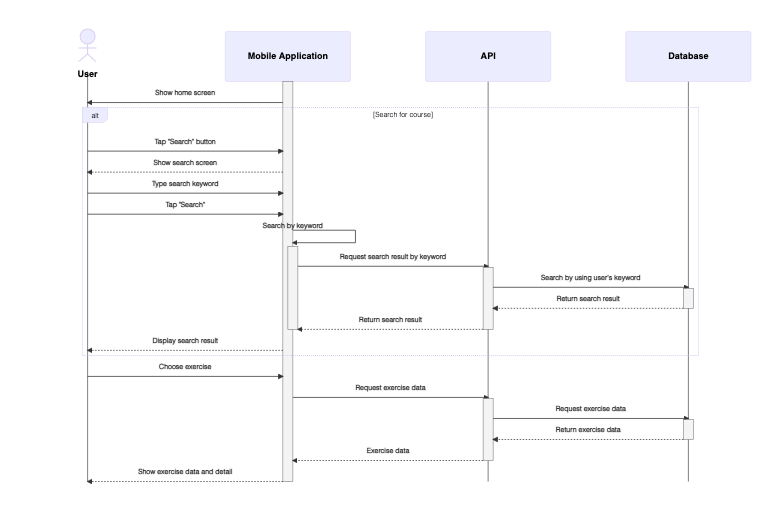
\includegraphics[width=\textwidth]{chapter_3/sequence/Exercise Course Selection-1.md.png}
    \caption{การทำงานในส่วนการเลือกคอร์สออกกำลังกาย}
\end{figure}

\begin{figure}
    \makebox[\textwidth][c]{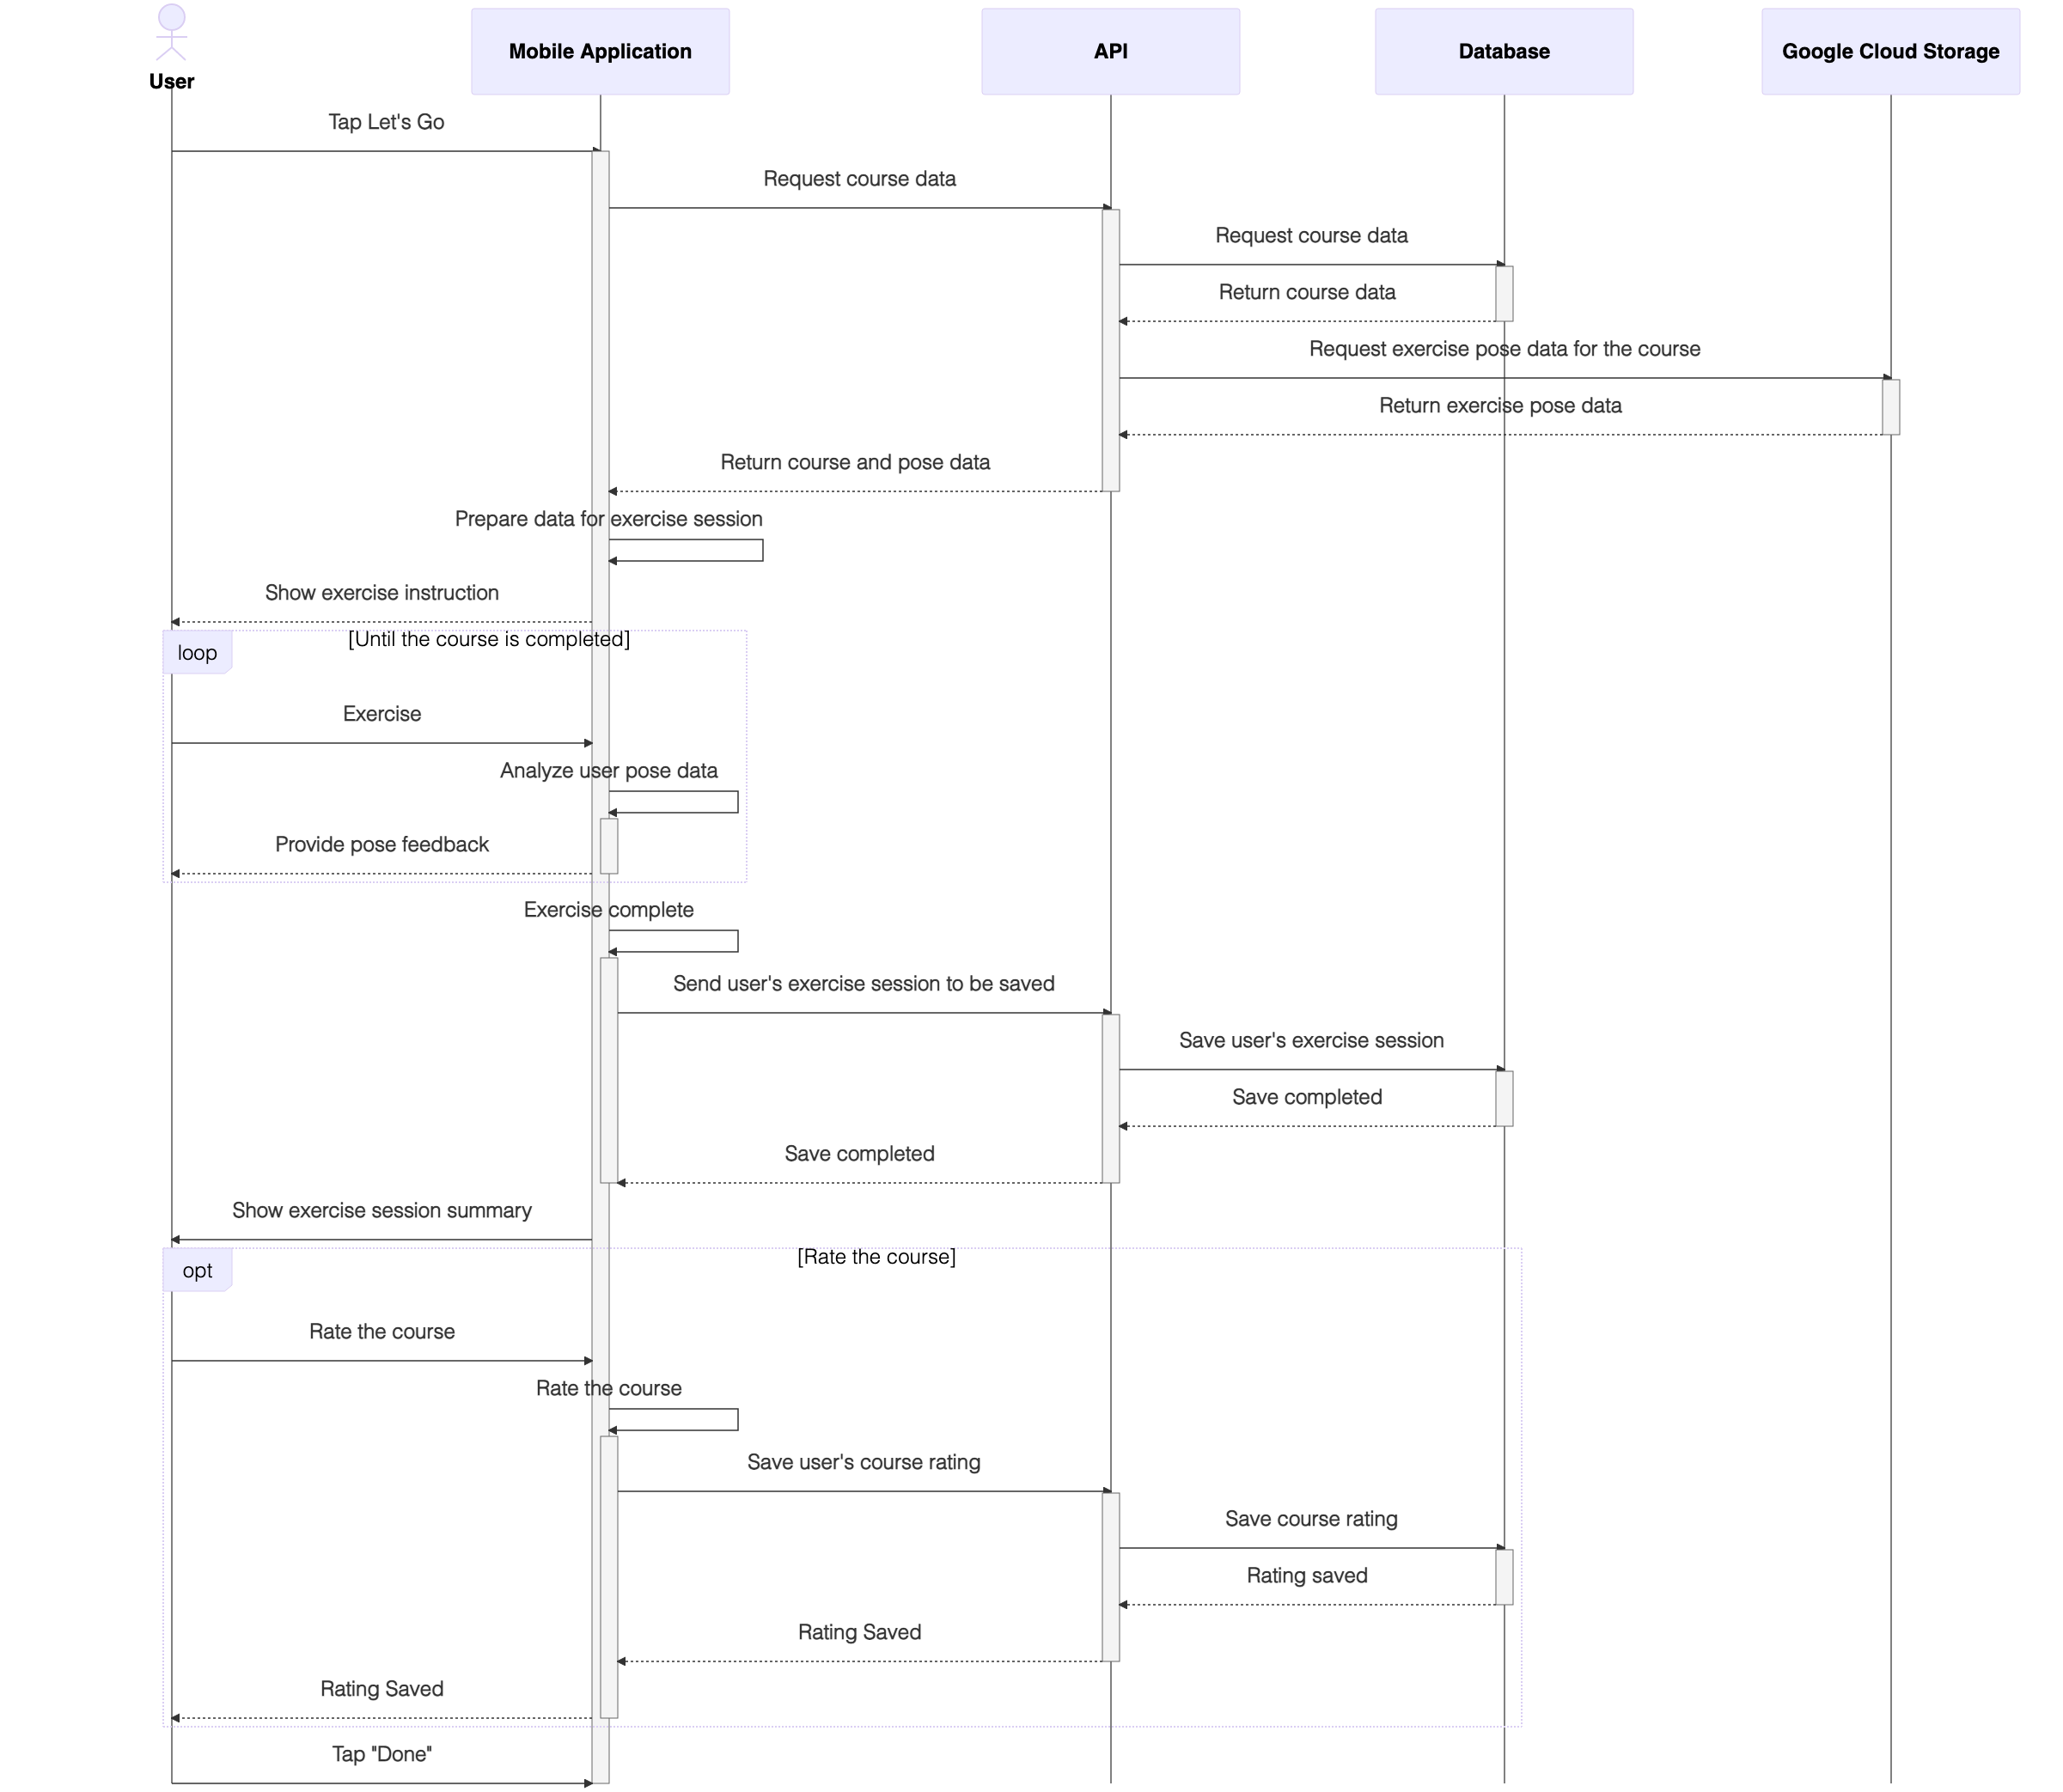
\includegraphics[width=\paperwidth - 3cm]{chapter_3/sequence/Exercise-1.md.png}}
    \caption{การทำงานในส่วนการออกกำลังกาย}
\end{figure}

\begin{figure}
    \makebox[\textwidth][c]{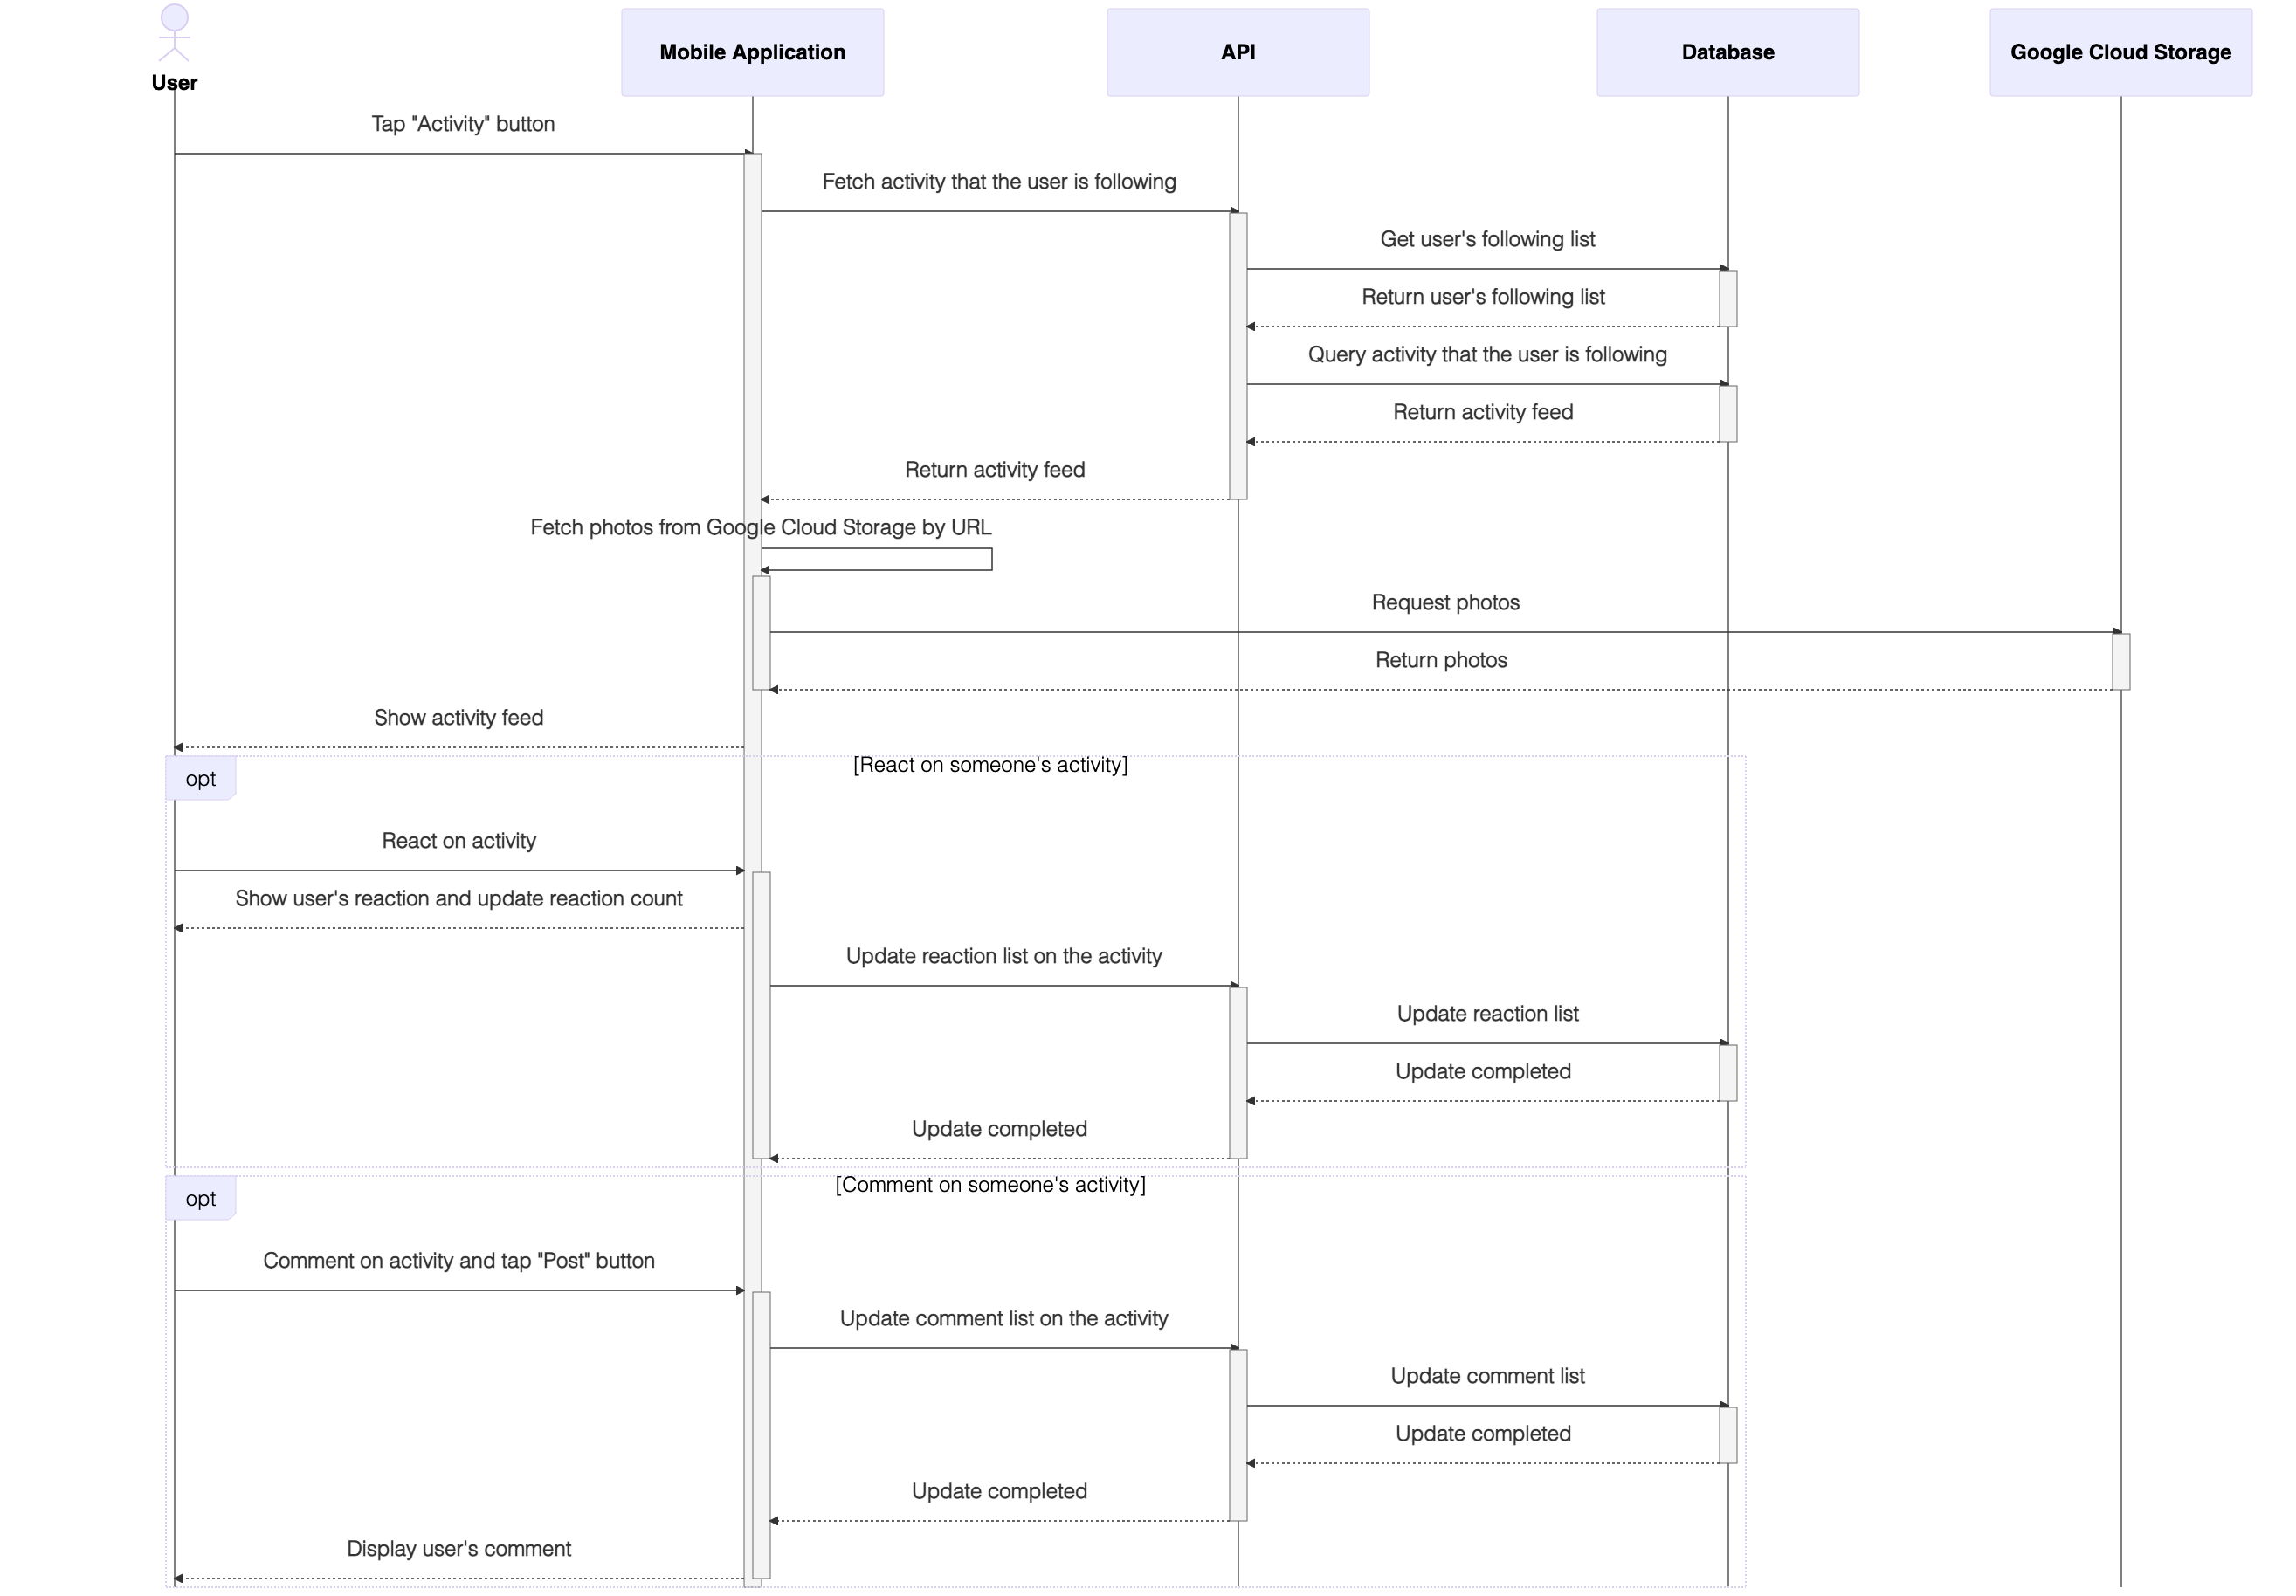
\includegraphics[width=\paperwidth - 3cm]{chapter_3/sequence/Activity-1.md.png}}
    \caption{การทำงานในส่วนกิจกรรมของผู้ใช้}
\end{figure}

\begin{figure}
    \makebox[\textwidth][c]{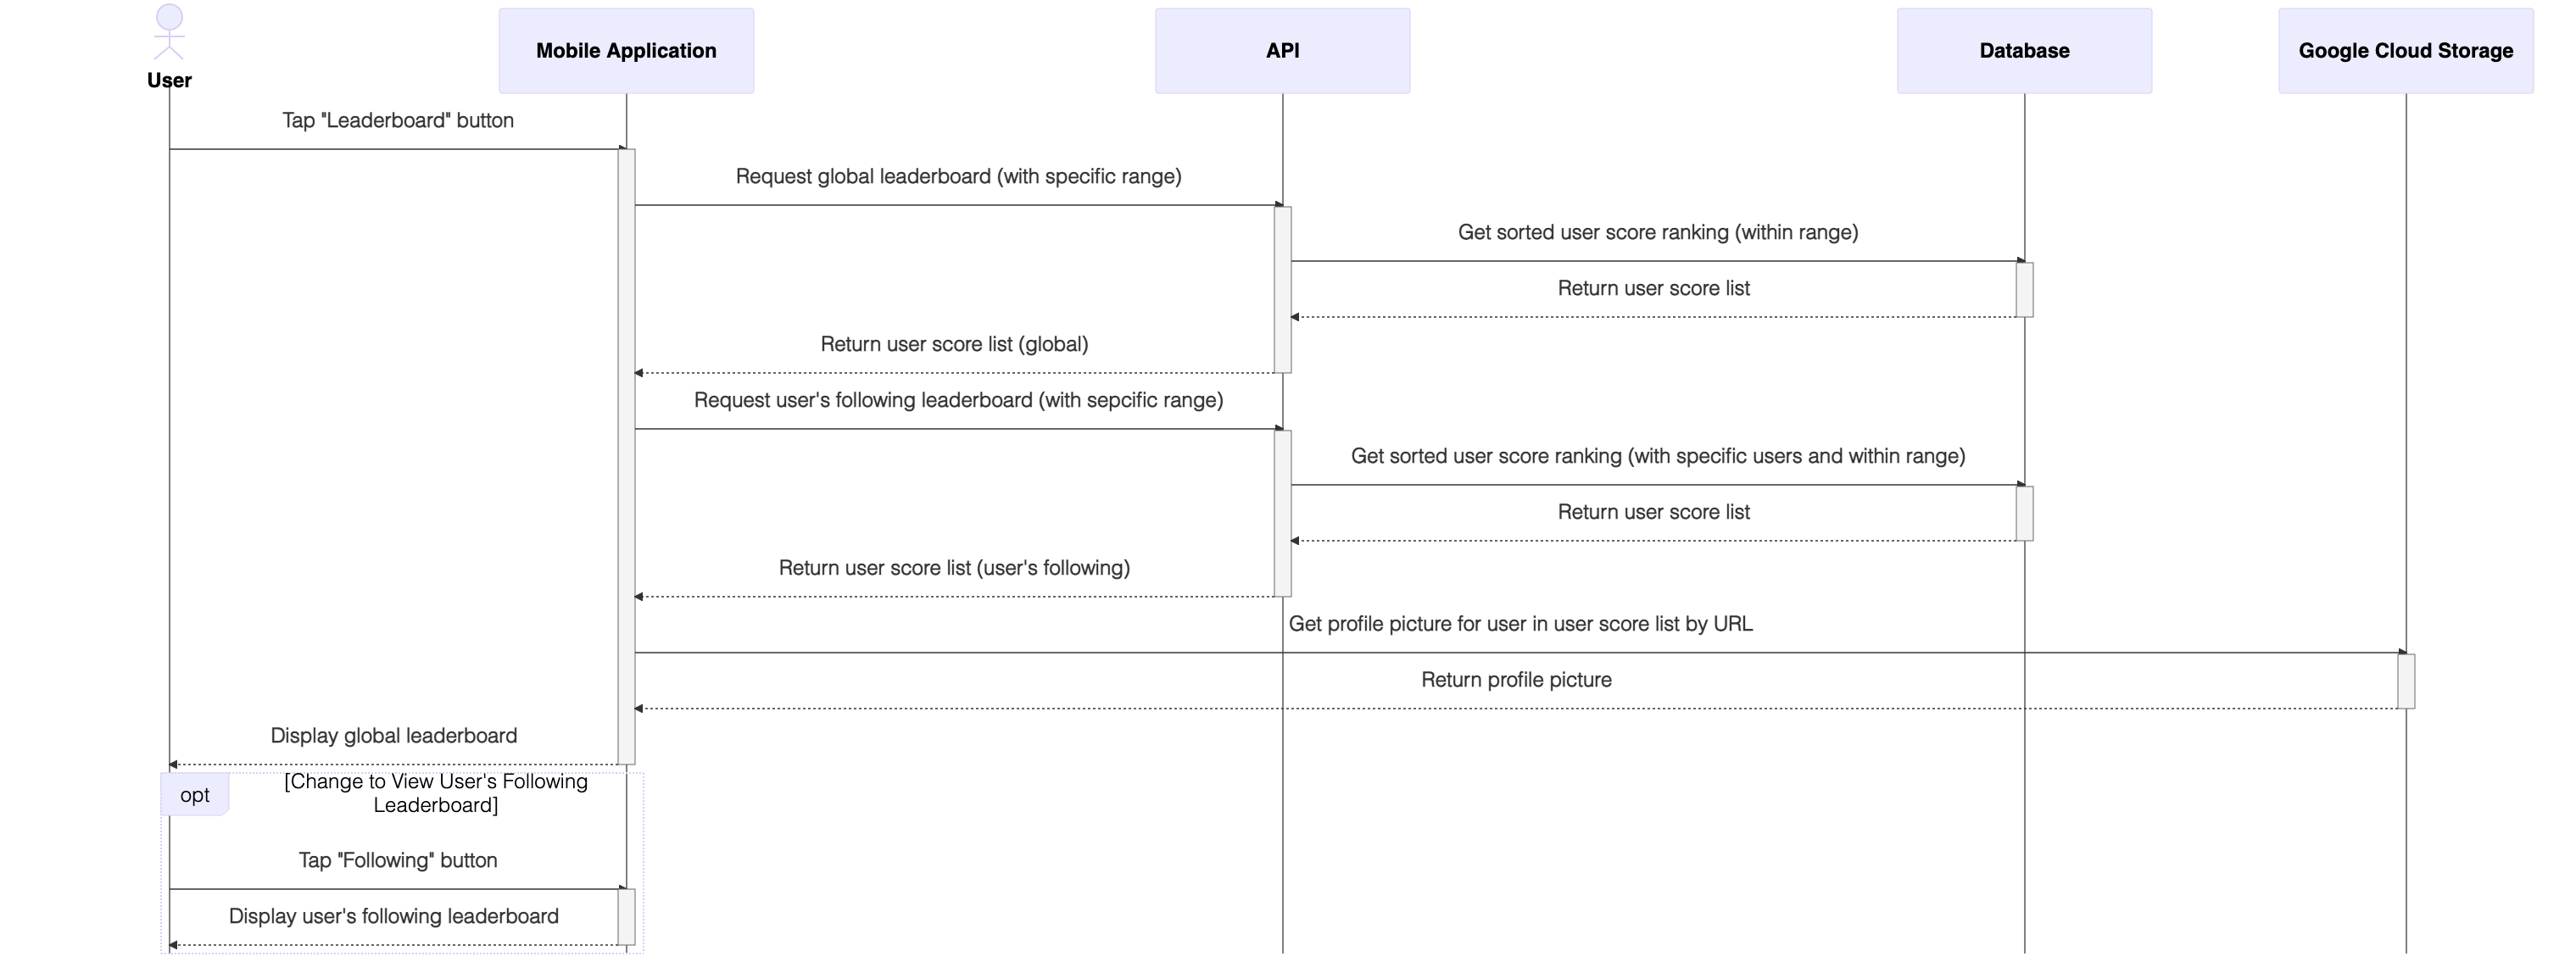
\includegraphics[width=\paperwidth - 3cm]{chapter_3/sequence/Leaderboard-1.md.png}}
    \caption{การทำงานในส่วนตารางคะแนน Leaderboard}
\end{figure}

\begin{figure}
    \makebox[\textwidth][c]{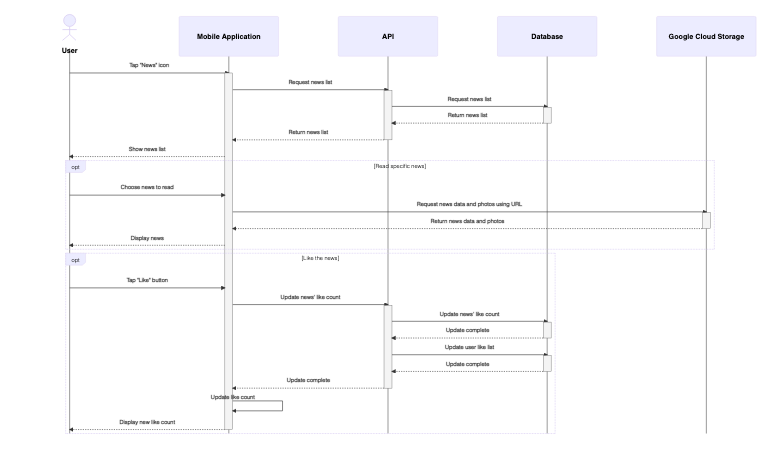
\includegraphics[width=\paperwidth - 3cm]{chapter_3/sequence/News-1.md.png}}
    \caption{การทำงานในส่วนข้อมูลข่าวสารของแอปพลิเคชัน}
\end{figure}

\begin{figure}
    \makebox[\textwidth][c]{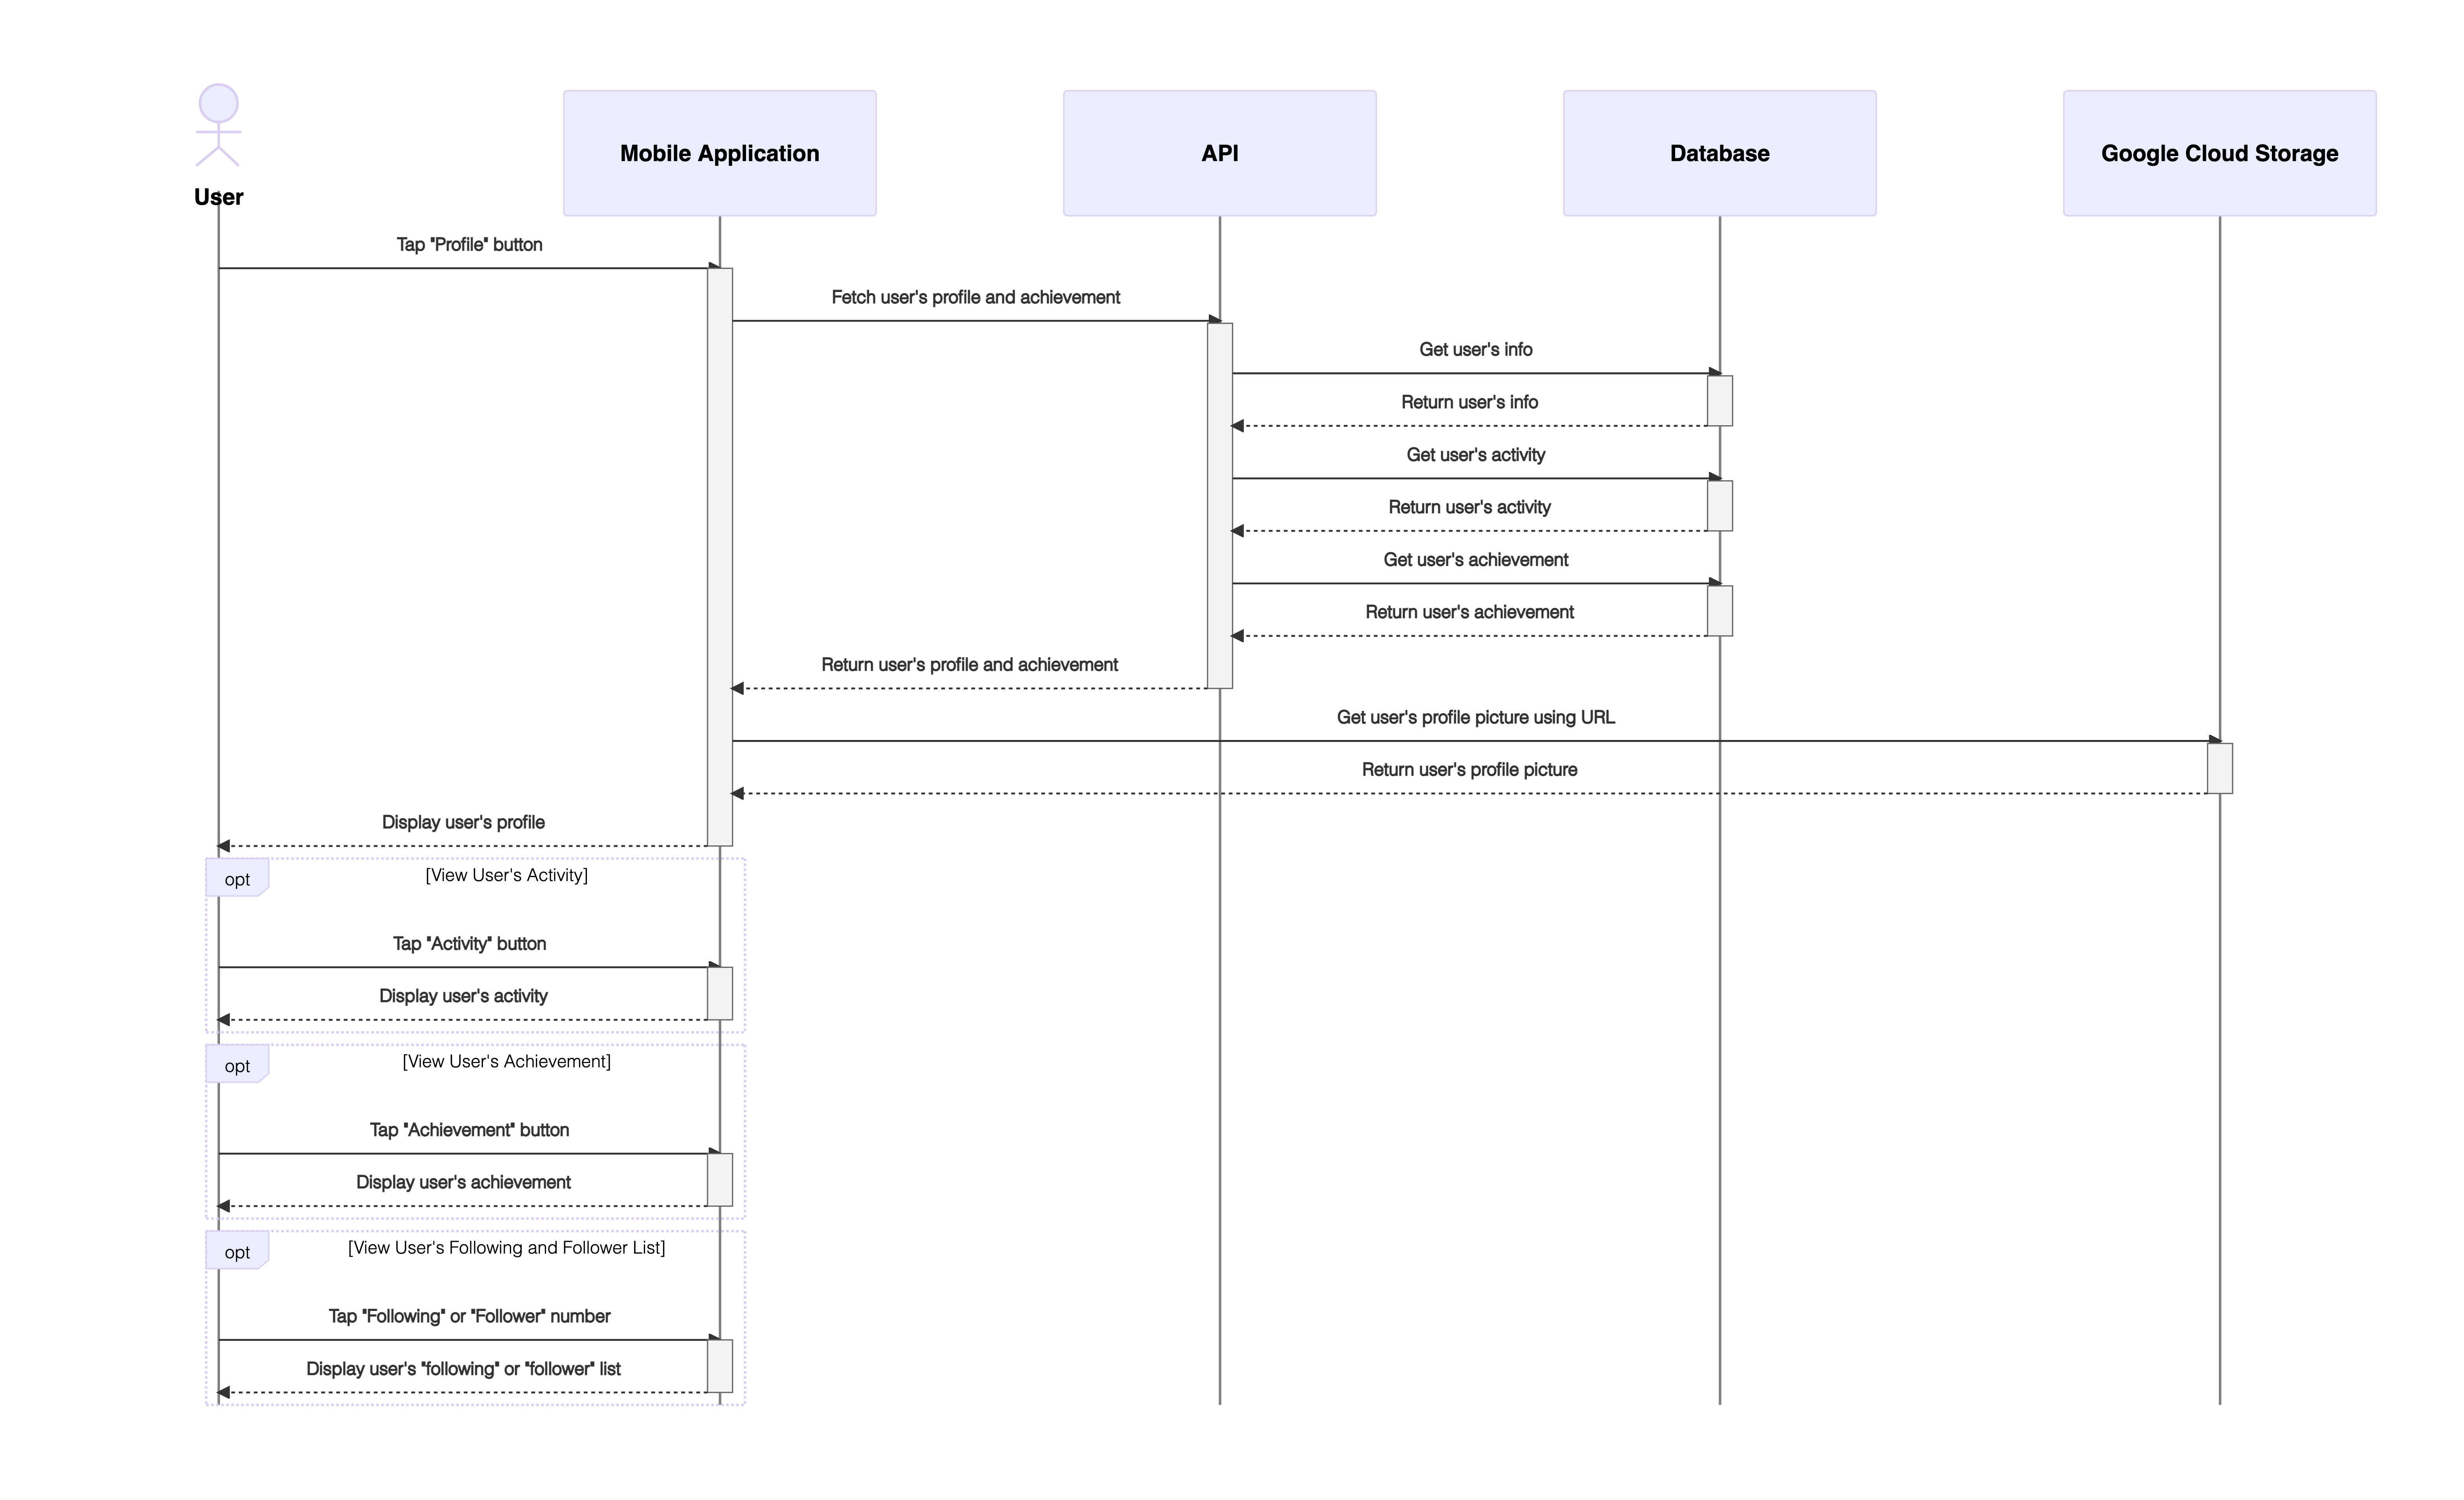
\includegraphics[width=\paperwidth - 3cm]{chapter_3/sequence/User Profile-1.md.png}}
    \caption{การทำงานในส่วนข้อมูลของผู้ใช้}
\end{figure}

\begin{figure}
    \makebox[\textwidth][c]{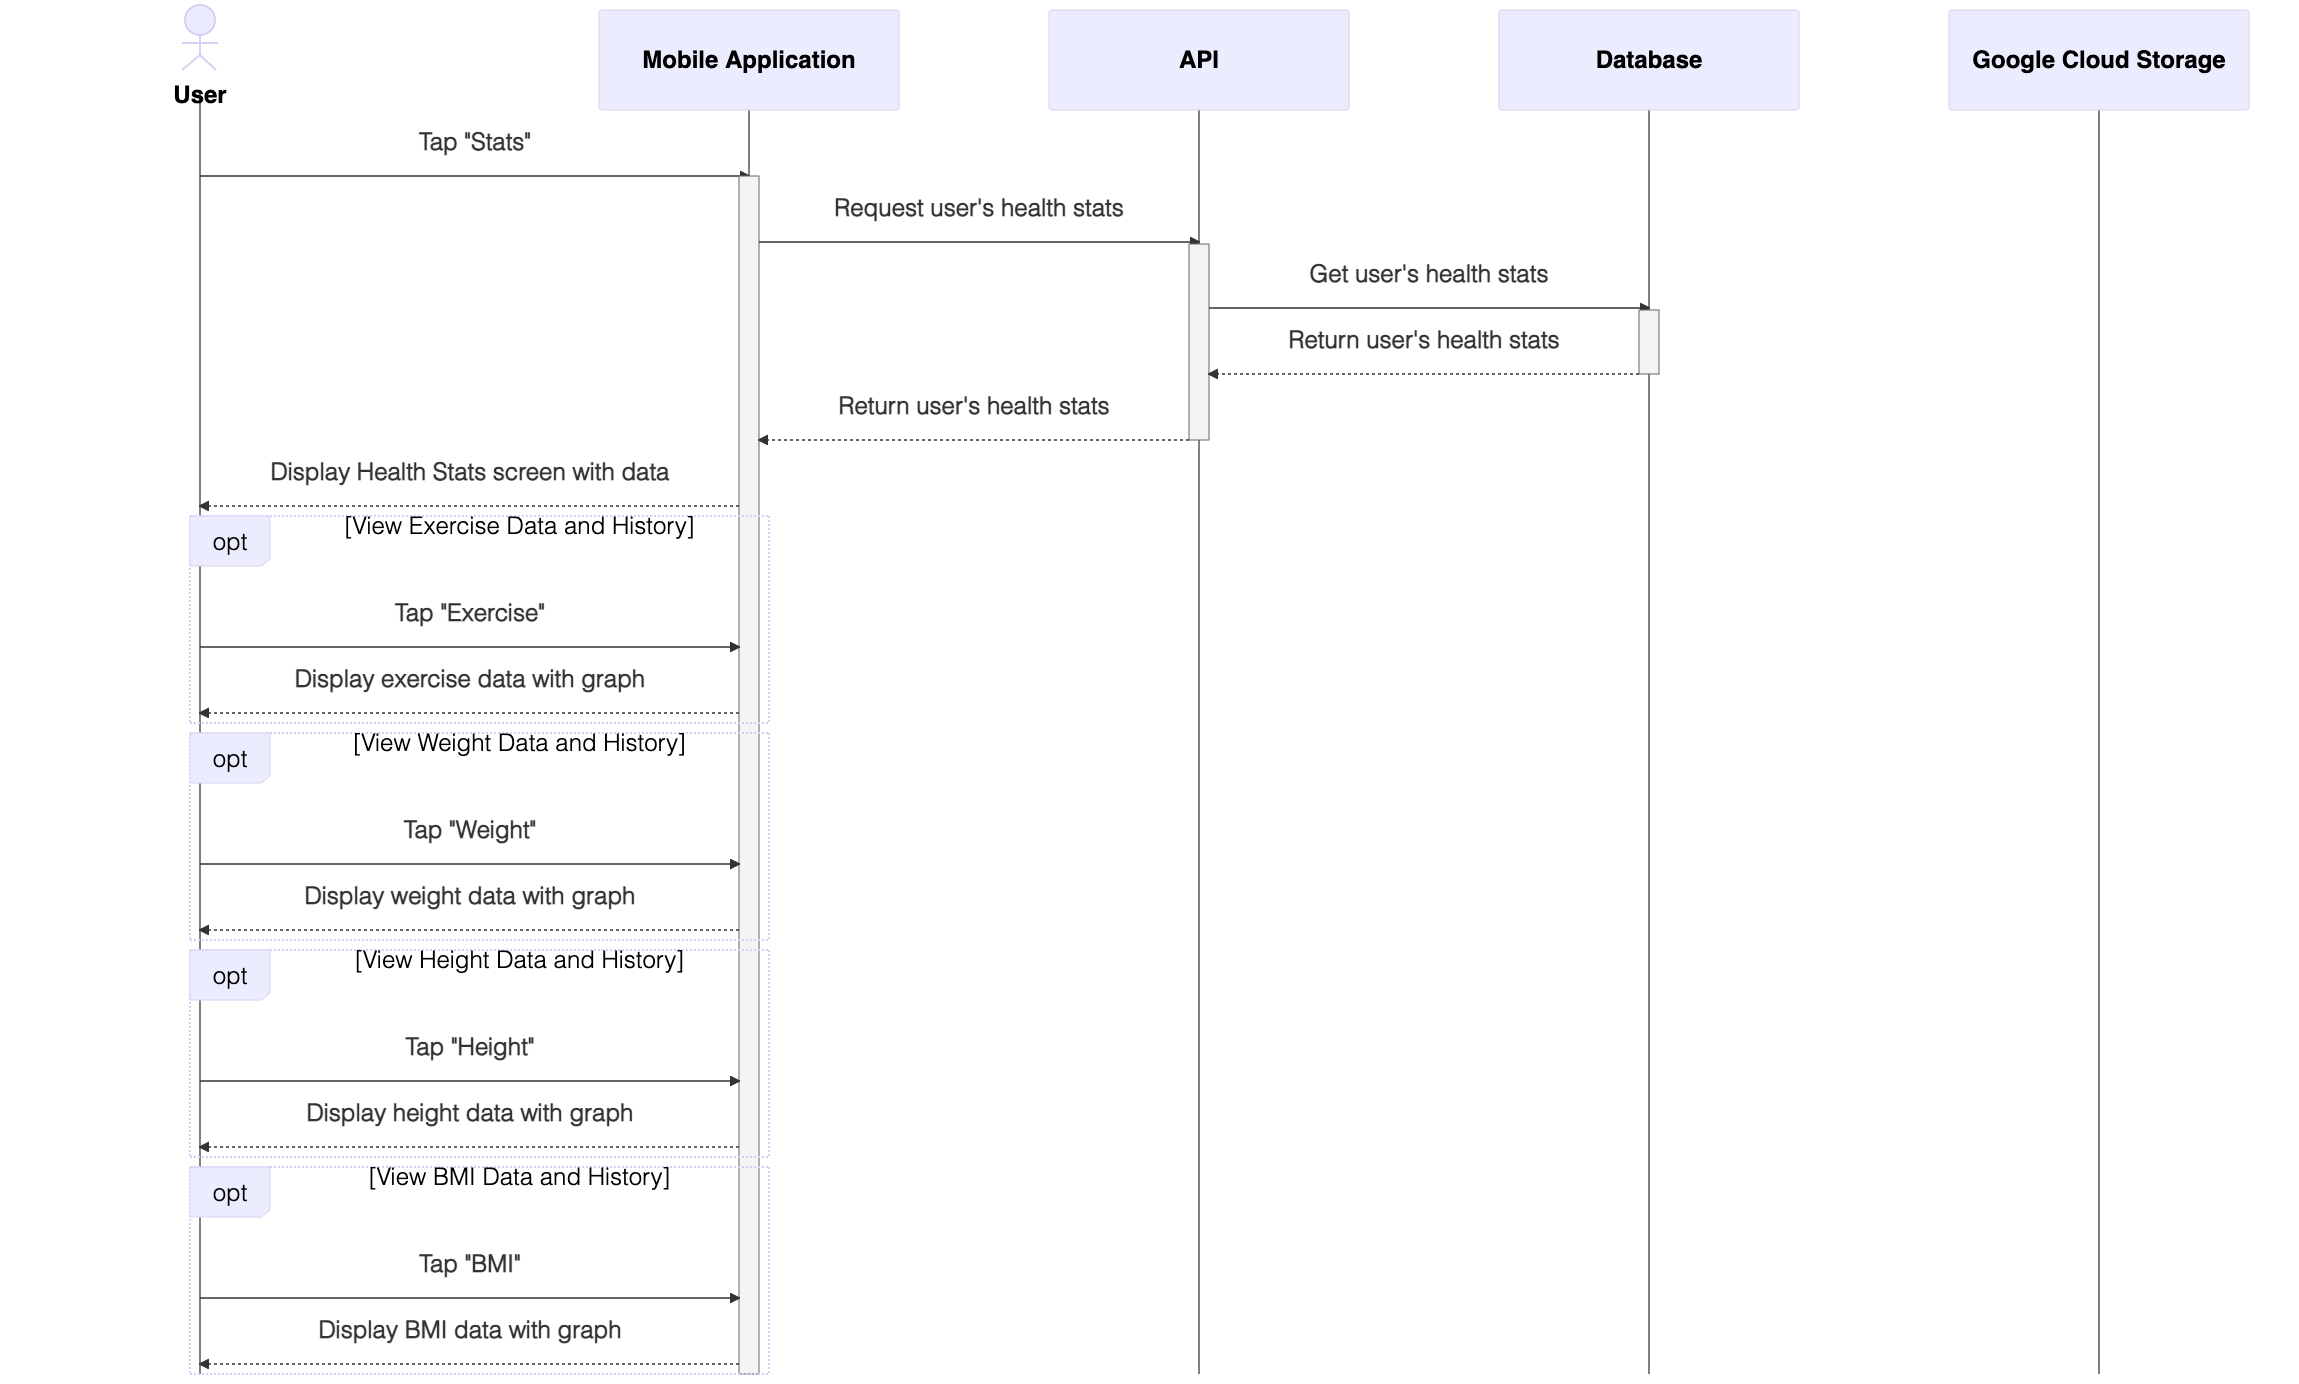
\includegraphics[width=\paperwidth - 3cm]{chapter_3/sequence/View Personal Health Stats-1.md.png}}
    \caption{การทำงานในส่วนข้อมูลสุขภาพของผู้ใช้}
\end{figure}

\begin{figure}
    \makebox[\textwidth][c]{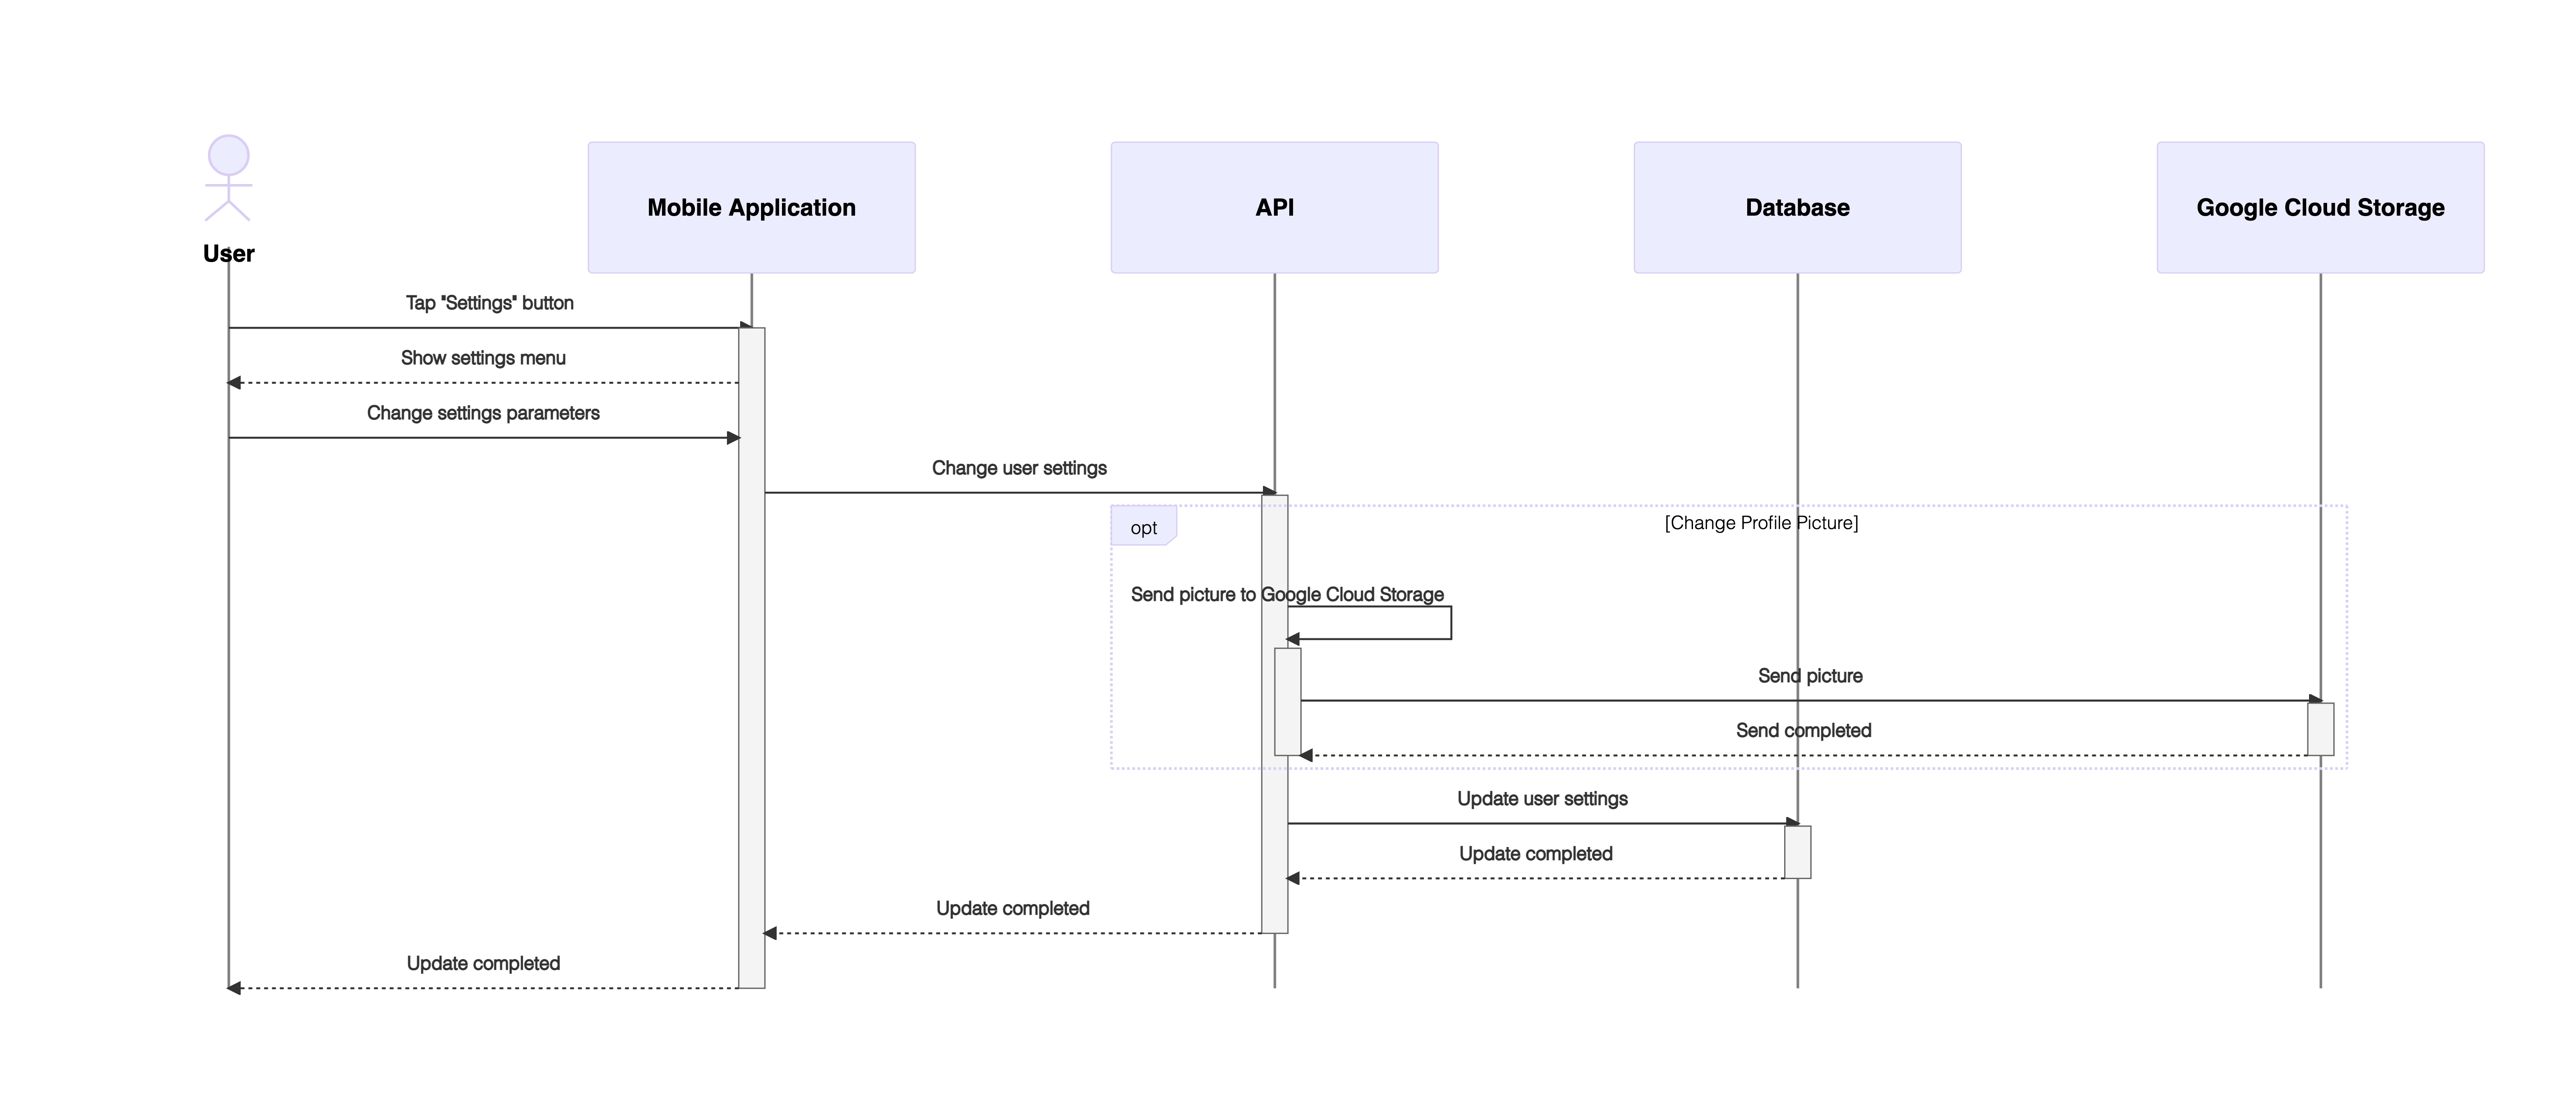
\includegraphics[width=\paperwidth - 3cm]{chapter_3/sequence/User Settings-1.md.png}}
    \caption{การทำงานในส่วนการตั้งค่าบัญชีผู้ใช้}
\end{figure}

\clearpage